\section{Linguistic Linked Open Data: Building the Cloud}

Recent years have seen not only a number of approaches to provide linguistic data as Linked Data, but also the emergence of larger initiatives that aim at interconnecting these resources.
Among these, the Open Linguistics Working Group (OWLG) of the Open Knowledge Foundation (OKFN) has spearheaded the creation of 
new data and the republishing of existing linguistic resources as part of the emerging Linguistic Linked Open Data (LLOD) cloud. 
As the OWLG organizes the LDL workshop series as a vehicle to facilitate this process, we would like to take the chance to unveil the revised cloud diagram on the occasion of LDL-2014.

\subsection{The LLOD Cloud}

Aside from benefits arising from the actual \emph{linking} of linguistic resources, various linguistic resources from very different fields have been provided in RDF and related standards in the last decade. In particular, this is the case for \textbf{lexical resources} (Fig.\ \ref{figI18nLOD}, \textsc{lexicon}), e.g., WordNet \citep{gangemi2003ontowordnet}, which represent a cornerstone of the Semantic Web and which are firmly integrated in the Linked Open Data (LOD) cloud. In a broader sense, also general knowledge bases from the LOD such as the DBpedia have been rendered as lexical resources, because of their immanent relevance for Natural Language Processing tasks such as Named Entity Recognition or Anaphora Resolution. Other types of linguistically relevant resources with less importance to AI and Knowledge Representation, however, are not a traditional part of the LOD cloud and motivate the creation of a sub-cloud dedicated to linguistic resources.

As such, the Linked Data paradigm also facilitates the management of information about language (Fig.\ \ref{figI18nLOD}, \textsc{language\_description}), i.e., linguistic terminology and linguistic databases. \textbf{Terminology repositories} serve an important role to establish conceptual interoperability between language resources. If resource-specific annotations or abbreviations are expanded into references to repositories of linguistic terminology and/or metadata categories, linguistic annotations, grammatical features and metadata specifications become more easily comparable. %Linguistic databases and annotated corpora linked to shared terminology repositories may help researchers from one particular community, say, NLP, to access and to re-use resources built up in the context of another linguistic sub-discipline, e.g., typology. 
Important repositories developed by different communities include GOLD \citep{farrar-langendoen03} and ISOcat \citep{wright2004global,windhouwer-wright2012}, yet, only recently these terminology repositories were put in relation with each other using Linked Data principles and with linguistic resources, e.g., within the OLiA architecture \citep{chiarcos-2012-olia-lrec}.
\textbf{Linguistic databases} are a particularly heterogeneous group of linguistic resources; they contain complex and manifold types of information, e.g., feature structures that represent typologically relevant phenomena, along with examples for their illustration and annotations (glosses) and translations applied to these examples (structurally comparable to corpus data), or word lists (structurally comparable to lexical-semantic resources). RDF as a generic representation formalism is thus particularly appealing for this class of resources.

Finally, for \textbf{linguistic corpora} (Fig.\ \ref{figI18nLOD}, \textsc{corpora}), the potential of the Linked Data paradigm for modeling, processing and querying of corpora is immense, and RDF conversions of semantically annotated corpora have been proposed early \citep{burchardt2008formalising}. \index{RDF (Resource Description Framework)}RDF provides a graph-based data model as required for the interoperable representation of arbitrary kinds of annotation \citep{bird01,ide-suderman07-graf}, and this flexibility makes it a promising candidate for a general means of representation for corpora with complex and heterogeneous annotations. \index{RDF (Resource Description Framework)}RDF does not only establish interoperability between annotations within a corpus, but also between corpora and other linguistic resources \citep{chiarcos-2012-ldl-powla}. In comparison to other types of linguistic resources, corpora are currently underrepresented in the LLOD cloud, but the development of schemes for corpora and/or NLP annotations represents an active line of research \citep{chiarcos2012-eswc-powla,hellmann-2012-ekaw} also addressed in the workshop.

%We apply the following criteria for a new linguistic resource to be included in the LLOD cloud diagram:
%(1) The data is resolvable through HTTP, (2) it is provided as RDF, (3) it contains links to another data set in the diagram, and (4) the entire data set must be available. ...

\begin{figure*}[t]
 \begin{center}
% \includegraphics[width=0.97\textwidth]{images/LODLinguistics.jpg}
% \includegraphics[width=0.97\textwidth]{images/llod}
 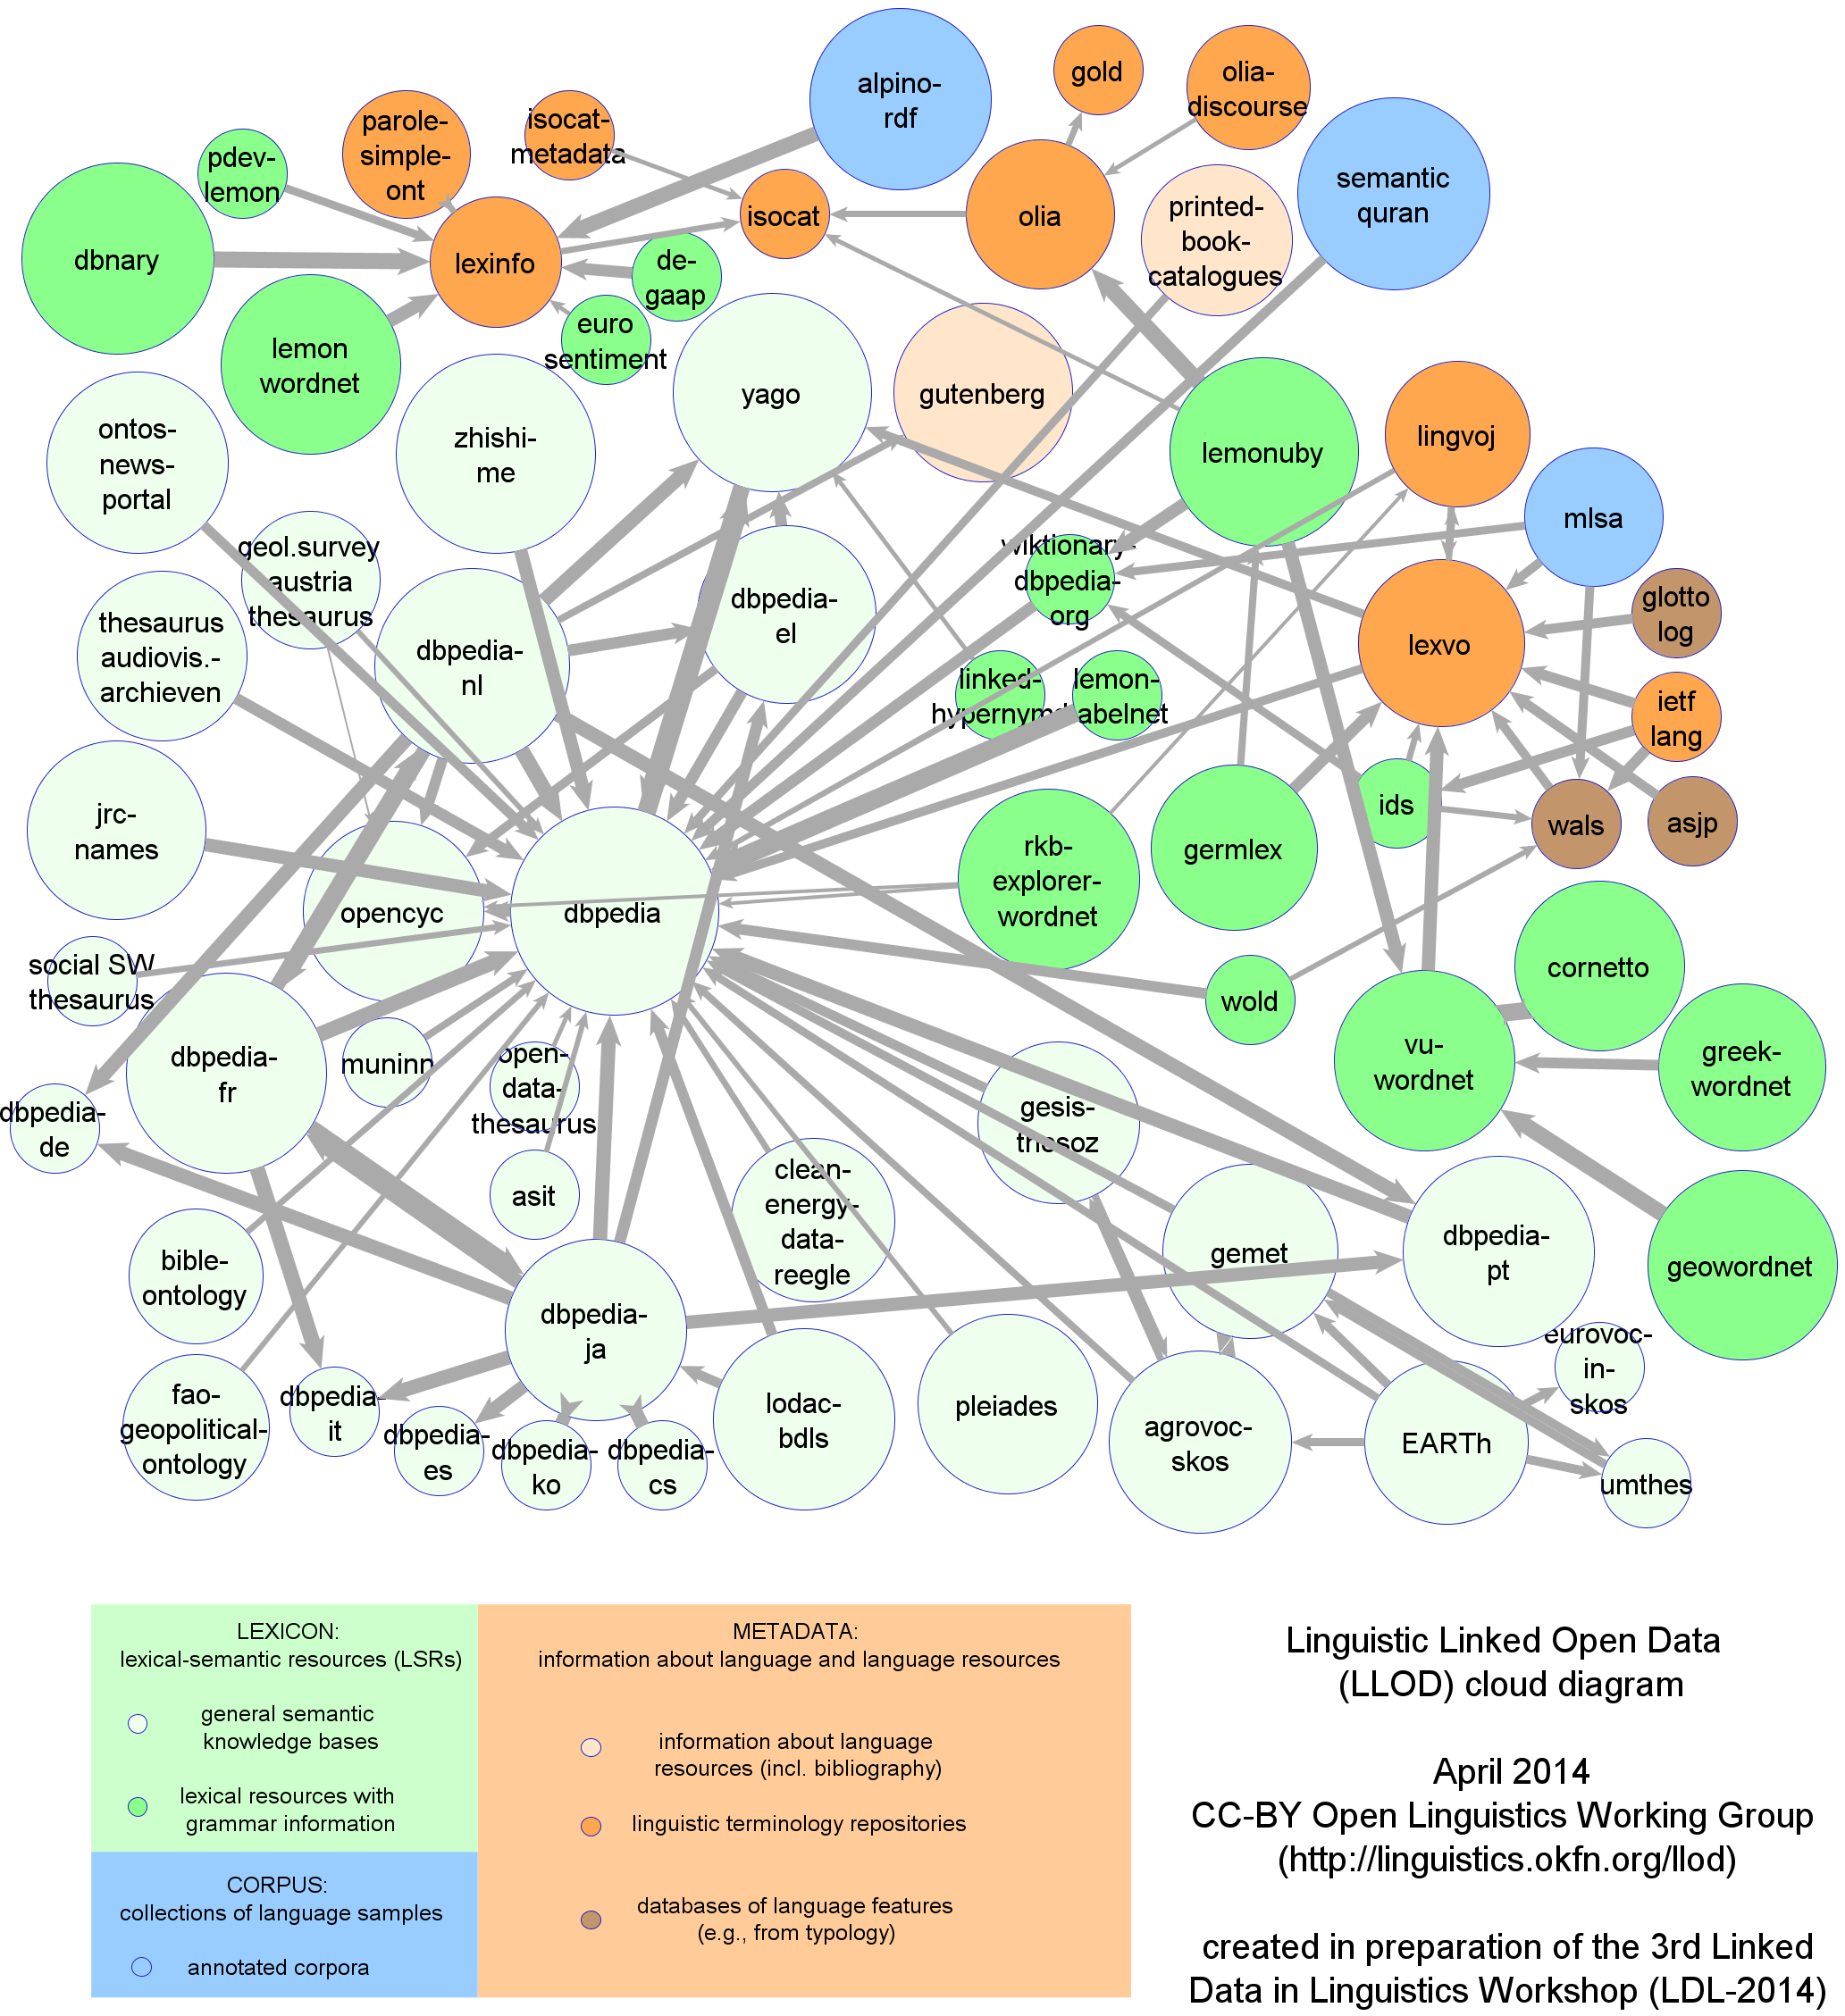
\includegraphics[width=0.8\textwidth]{llod-colored.png}
 \end{center}
\caption{Linguistic Linked Open Data cloud as of September 2013.}
\label{figI18nLOD}
\end{figure*}

\subsection{Recent Developments}


At the moment, we have 107 data sets, we decided to restrict the cloud to resources whose links are specified in Datahub.io.

hence linked datasets only


The first draft of the LLOD diagram has been sketched ...

Since LDL-2013, the categories have been increasingly clarified

Novel data sets include

\subsection{Behind LDL-2014}

% The LDL workshop series and LDL-2014 are organized by the Open Linguistics Working Group, and supported by LIDER & QTLeap

% An important vehicle for this process are workshops organized by the OWLG. 
% These include the Linked Data in Linguistics workshop series (March 2012 in Frankfurt am Main, Germany; Sep 2013 in Pisa, Italy; May 2014 in Reykjavik, Iceland) which bring together researchers from linguistics, NLP and Semantic Web, 
% as well as more specialized events such as a workshop on Multilingual Linked Open Data for Enterprises (MLODE-2012: Sep 2012 in Leipzig, Germany) or the 
% theme session on Linked Data in Linguistic Typology (at the 10th Biennial Conference of the Association for Linguistic Typology, ALT-2013, Aug 2013 in Leipzig, Germany), as well as presentations, panels and informal meetings at selected conferences.

% Yet, before giving an overview over the contributions to LDL-2014, 
% Related initiatives include the W3C Ontology-Lexica Community Group that is seeking to develop standard models for representing and publishing (ontology-) lexica and other lexical resources as RDF, and th


% Since LDL-2013, the  


% The LDL workshop series is organized by the 

% , culminating on the creation of a Linguistic Linked Open Data (LLOD) cloud, i.e., a Linked Open Data (sub-)cloud of linguistic resources.



% The 

% LDL-2013 is organized in the context of two recent community efforts, the Open Linguistics Working Group  (OWLG), and the W3C Ontology-Lexica Community Group (OntoLex). 


The LLOD cloud is a result of a coordinated effort of the {\bf Open Linguistics Working Group (OWLG)},\footnote{\url{http://linguistics.okfn.org}} a network open to anyone interested in linguistic resources and/or the publication of these under an open license. The OWLG is a working group of the Open Knowledge Foundation (OKFN),\footnote{\url{http://okfn.org/}} a community-based non-profit organization promoting open knowledge (i.e., data and content that is free to use, re-use and to be distributed without restriction).
%The OWLG adopts OKFN's principles, definitions and infrastructure as far as they are relevant for linguistic data. The OKFN defines standards and develops tools that allow anyone to create, discover and share open data. The Open Definition of the OKFN states that ``openness'' refers to: ``A piece of content or data [that] is open if anyone is free to use, reuse, and redistribute it -- subject only, at most, to the requirement to attribute and share-alike.''\footnote{\url{http://opendefinition.org}}
%The Open Definition is accompanied by a list of compliant licenses.
%One important aspect here is that openness should not constrain the use of data provided under these licenses, e.g., its commercial use, and that it should allow to complement these with proprietary resources. Adopting this understanding of openness for the LLOD cloud warantees that the resources contained in the cloud are available under \emph{any circumstances}.

%One tool that the OKFN provides is \textbf{CKAN},\footnote{\url{http://ckan.org/}} a catalog system for open data sets. CKAN is an open-source data portal software developed to easily publish, find and reuse open content and data, particularly in ways that are also machine automatable. The OKFN also hosts various working groups addressing problems of open data in different domains. Currently, there are 18 OKFN \textbf{working groups} covering fields as diverse as government data, economics, archeology, text books and cultural heritage. The OKFN organizes various events, such as the Open Knowledge Conference (OKCon), and facilitates the exchange of ideas between different working groups. The vision of the OKFN is a world in which open knowledge is ubiquitous. In this paper, we apply the aims of open knowledge to data in the field of linguistics.

Since its formation in 2010, the Open Linguistics Working Group has grown steadily. One of our primary goals is to attain openness in linguistics through:

\begin{enumerate}
\item Promoting the idea of open linguistic resources,
\item Developing the means for the representation of open data, and
\item Encouraging the exchange of ideas across different disciplines.
\end{enumerate}

\noindent 
%Publishing linguistic data under open licenses is an important issue in academic research, as well as in the de\-ve\-lop\-ment of applications. We see increasing support for this in the linguistics community \citep{Pederson:2008}, and there are a growing number of resources published under open licenses \citep{meyers2007shared}. There are many reasons for publishing resources under open licenses: for instance, freely available data can be more easily re-used, double investments can be avoided, and results can be replicated. Also, other researchers can build on this data, and subsequently refer to the publications associated with it. Nevertheless, a number of ethical, legal and sociological problems are associated with open data,\footnote{
%For example, complex copyright situations may arise if one resource (say, a lexicon) was developed on the basis of another resource (say, a newspaper archive), and researchers are uncertain whether the examples from the original newspaper contained in the lexicon violate the original copyright. Ethical problems may arise if a data base of quotations from a newspaper is linked to a data base of speakers, and this data base is further connected with, say, obituaries from the same newspaper. Even if this was done only in order to study generation-specific language variation, one may wonder whether such a accumulation of information violates the privacy of the people involved.
%}
%and the technologies that establish interoperability (and thus, re-usability) of linguistic resources are still under de\-ve\-lop\-ment. 
%
The OWLG represents an open forum for interested individuals to address these and related issues.
At the time of writing, the group consists of about 100 people from 20 different countries.
Our group is relatively small, but continuously growing and sufficiently heterogeneous. It includes
people from library science, typology, historical linguistics, cognitive science, computational linguistics, and information technology; the ground for fruitful interdisciplinary discussions has been laid out.
One concrete result emerging out of collaborations between a large number of OWLG members is the LLOD cloud as already sketched above.
%Independent research activities of many community members involve the application of RDF/OWL to represent linguistic corpora, lexical-semantic resources, terminology repositories and metadata collections about linguistic data collections and publications, and to many of them, the Linked Open Data paradigm represents a particularly appealing set of technologies. Within the OWLG, these activities converged towards building the cloud. 

The emergence of the LLOD cloud out of a set of isolated resources was accompanied and facilitated by a series of \textbf{workshops and publications} organized under the umbrella of the OWLG, including the Open Linguistics track at the Open Knowledge Conference (OKCon-2010, July 2010, Berlin, Germany), the First Workshop on Linked Data in Linguistics (LDL-2012, March 2012, Frankfurt am Main, Germany), the Workshop on Multilingual Linked Open Data for Enterprises (MLODE-2012, September 2012, Leipzig, Germany), the Linked Data for Linguistic Typology track at ALT-2012 (September 2013, Leipzig, Germany). Plans to create a LLOD cloud were first publicly announced at LDL-2012, and subsequently, a first instance of the LLOD materialized as a result of the MLODE-2012 workshop, its accompanying hackathon and the data postproceedings that will appear as a special issue of the Semantic Web Journal (SWJ). The Second Workshop on Linked Data in Linguistics (LDL-2013) continues this series of workshops. In order to further contribute to the integration of the field, it is organized as a joint event of the OWLG and the W3C Ontology-Lexica Community Group.

The \textbf{Ontology-Lexica Community (OntoLex) Group}\footnote{\url{http://www.w3.org/community/ontolex}} was founded  in September 2011 as a W3C Community and Business Group. It aims to produce specifications for a lexicon-ontology model that can be used to provide rich linguistic grounding for domain ontologies.
Rich linguistic grounding include the representation of morphological, syntactic properties of lexical entries as well as the syntax-semantics interface, i.e., the meaning of these lexical entries with respect to the ontology in question. An important issue herein will be to clarify how extant lexical and language resources can be leveraged and reused for this purpose. As a byproduct of this work on specifying a lexicon-ontology model, it is hoped that such a model can become the basis for a web of lexical linked data: a network of lexical and terminological resources that are linked according to the Linked Data Principles forming a large network of lexico-syntactic knowledge.

The OntoLex W3C Community Group has been working for more than a year on realizing a proposal for a standard ontology lexicon model, currently discussed under the the designation \emph{lemon}. As the core specification of the model is almost complete, the group started to develop of additional modules for specific tasks and use cases, and some of these are presented at LDL-2013.

